% !TeX encoding = UTF-8
\documentclass[aspectratio=169]{beamer}
\useoutertheme[progressbar=frametitle]{metropolis}
\useinnertheme{metropolis}
\definecolor{nabgray}{rgb}{0.6,0.59,0.61}
\usecolortheme[named=nabgray]{structure}

\usepackage{tikz}
\usepackage[utf8]{inputenc}
\usepackage[spanish]{babel}
\usepackage{fontspec}
\setmonofont{JetBrains Mono}
\setmainfont{Roboto}
\setsansfont{Roboto}

\usepackage{smartdiagram}
\usepackage{qtree}
\usepackage{verbatim}
\usepackage{svg}
\usepackage{graphicx}
\usepackage{color}

\definecolor{lightgray}{rgb}{0.95, 0.95, 0.95}
\definecolor{darkgray}{rgb}{0.4, 0.4, 0.4}
%\definecolor{purple}{rgb}{0.65, 0.12, 0.82}
\definecolor{editorGray}{rgb}{0.95, 0.95, 0.95}
\definecolor{editorOcher}{rgb}{1, 0.5, 0} % #FF7F00 -> rgb(239, 169, 0)
\definecolor{editorGreen}{rgb}{0, 0.5, 0} % #007C00 -> rgb(0, 124, 0)
\definecolor{orange}{rgb}{1,0.45,0.13}
\definecolor{olive}{rgb}{0.17,0.59,0.20}
\definecolor{brown}{rgb}{0.69,0.31,0.31}
\definecolor{purple}{rgb}{0.38,0.18,0.81}
\definecolor{lightblue}{rgb}{0.1,0.57,0.7}
\definecolor{lightred}{rgb}{1,0.4,0.5}
\usepackage{upquote}
\usepackage{listings}
\lstset{language=java,
	basicstyle=\footnotesize\ttfamily,
	keywordstyle=\footnotesize\color{blue}\ttfamily,
	escapeinside={<@}{@>}
}


\usebackgroundtemplate%
{%
	
\includegraphics[width=\paperwidth]{Images/Contenido}%
}


\title{Consideraciones al migrar un sistema tradicional hacia Cloud Native}
\author{Víctor Orozco}
\institute{Nabenik}
\date{\today}

\begin{document}





{
    \usebackgroundtemplate{
\includegraphics[width=\paperwidth]{Images/portada}}
    \setbeamercolor{frametitle}{fg=red}
    \usebeamercolor[fg]{normal text}
    \frame{\titlepage}
}

\begin{frame}{Cloud native}
Al migrar hacia nuevas tecnologías cloud -e.g. Serverless, BaaS, Microservicios- automáticamente van a conseguir escala -i.e. soportar más usuarios con menos dinero-  y lanzar más rápido.
\end{frame}


\begin{frame}{Cloud native}

\textbf{Enfoque} para la construcción de sistemas informáticos modernos sobre entornos dinámicos como nubes privadas y públicas.

	\begin{itemize}
		\item Sistemas reactivos
		\item 12 factores cloud native
        \item Design patterns
        \item Domain Driven Design
		\item Microservices chassis y/o service mesh
        \item Orquestación de contenedores, serverless, BaaS
        \item Nube
	\end{itemize}

\end{frame}


\begin{frame}{Cloud native}

	\begin{itemize}
		\item (Nos gustaría tener) Sistemas reactivos
		\item (Es posible con la metodología de) 12 factores Cloud Native
        \item (Usamos soluciones probadas mediante) design patterns
        \item (Fragmentamos el sistema mediante) Domain Driven Design
		\item (Implementamos los servicios con) Microservices chassis y/o service mesh
        \item (Hacemos despliegue) Mediante orquestación de containers, funciones serverless, BaaS
        \item (Contratamos)  Nube
	\end{itemize}

Un proceso de migración hacia Cloud Native es en si mismo un macro proyecto.

\end{frame}

{
	\usebackgroundtemplate{
\includegraphics[width=\paperwidth]{Images/separador}}
	\setbeamercolor{normal text}{fg=white}
	\setbeamercolor{frametitle}{fg=red}
	\usebeamercolor[fg]{normal text}
	\section{El proyecto de migración}
}

\begin{frame}{Cloud native - Experiencias previas}

	\begin{itemize}
    		\item Inicio
            	\begin{itemize}
                		\item Diagnostico de arquitectura y equipo de trabajo
                	\end{itemize}
    		\item Planificación
            	\begin{itemize}
                		\item Elaboración de hoja de ruta
                	\end{itemize}
            \item Ejecución
            	\begin{itemize}
                		\item Implementación
                		\item Adquisición
                        \item Capacitación
                        \item Programación
                	\end{itemize}
            \item Monitoreamiento y control
            	\begin{itemize}
                		\item Tecnológico: Evaluaciones de entregables, métricas de calidad
                        \item Proyecto: Presupuesto, plazos, viabilidad real de los entregables
                	\end{itemize}
    		\item Cierre
\begin{itemize}
                		\item Documentación viva
                        \item Mejoras futuras
                	\end{itemize}
    	\end{itemize}

\end{frame}


\begin{frame}{Inicio}
No más de dos reuniones exploratorias. En promedio 2 horas por reunión\\

Stakeholders que no pueden faltar:\\
\begin{itemize}
\item Arquitecto de software (Tech Lead, Dev. Sr.)
\item Jefe de infraestructura (Sysadmin principal, SRE)
\item Punto de contacto (generalmente el arquitecto de software o soluciones)
\end{itemize}

Preguntas clave:\\
\begin{itemize}
\item Motivación principal
\item Personal actual
\item Stack(s) tecnológicos 
\end{itemize}
\end{frame}

\begin{frame}{Planificación}
Revisión de arquitectura actual
\begin{itemize}
\item Datos importantes
\item Problemas
\item Propuesta macro de mejoras
\item Listado de acciones puntuales
\item Hoja de ruta con opciones (contratación, consultoria, tercerización, entrenamiento)
\item Contrato(s) basado(s) en entregables
\end{itemize}
\end{frame}

\begin{frame}{Planificación}
\begin{figure}
\centering
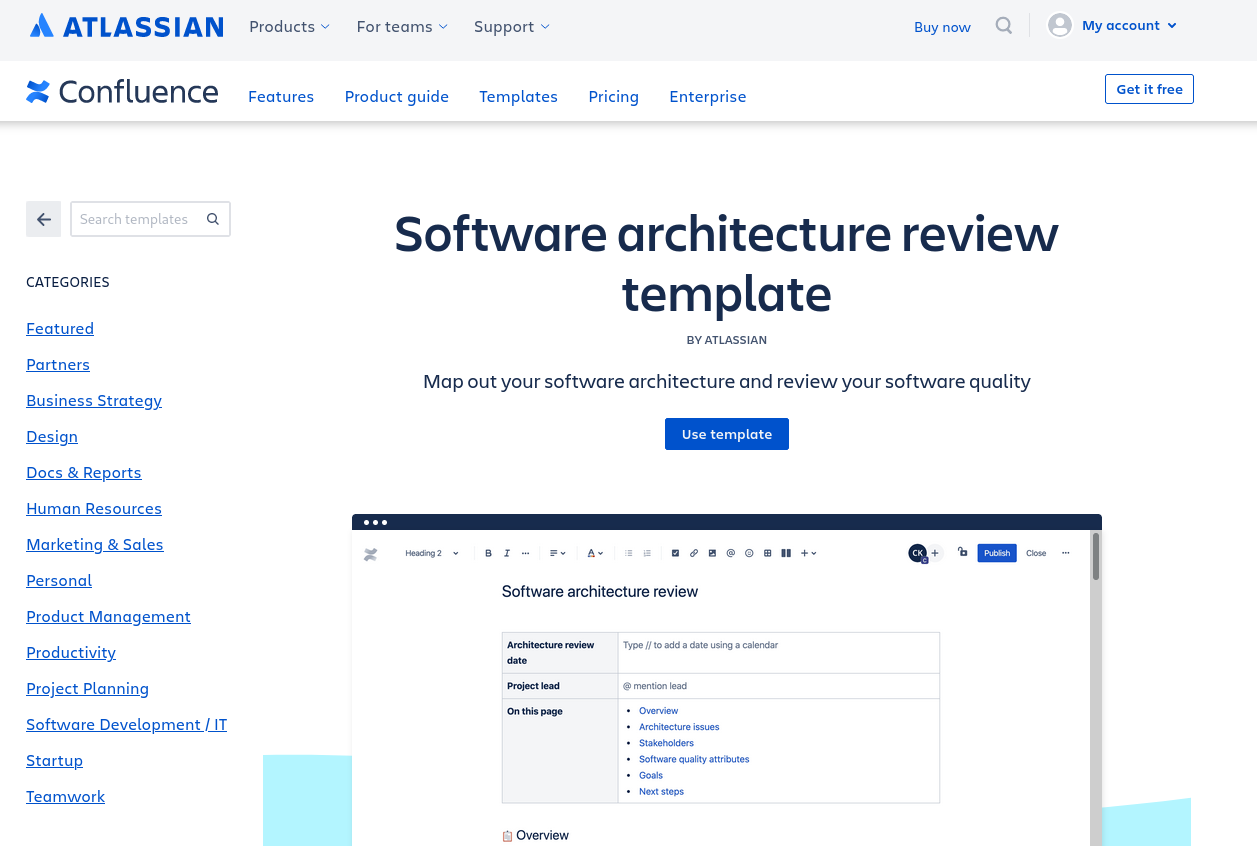
\includegraphics[width=\linewidth]{Images/atlassian}
\end{figure}
\end{frame}

\begin{frame}{Planificación}
\begin{figure}
\centering
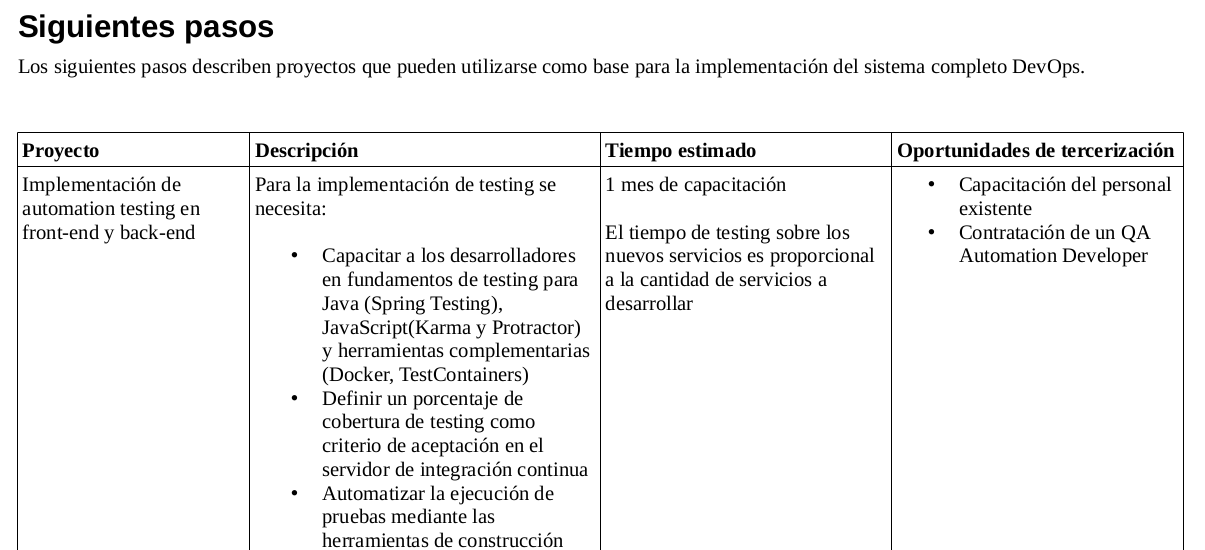
\includegraphics[width=0.8\linewidth]{Images/pasos}
\end{figure}
\end{frame}

\begin{frame}{Ejecución}
1-Punto de contacto, 2-Medio de comunicación inmediato, 3- Medio de comunicación no repudiable.


\begin{itemize}
    \item Cultura
        \begin{itemize}
        \item DevOps
        \item Test Driven Development
        \end{itemize}
    \item  Infraestructura
        \begin{itemize}
        \item Accesos remotos
        \item VCS, CI/CD
        \item Plataforma Cloud Native -e.g. Openshift, Kubernetes, Amazon EKS, Oracle Kubernetes Engine-
        \item Observabilidad -e.g. Linkerd, Prometheus, Grafana, ELK, alarmas-
        \end{itemize}
 \end{itemize}
 Idealmente realizar una presentación/transferencia de tecnología por entregable.
\end{frame}


\begin{frame}{Ejecución}
Todas estas etapas producirán \textbf{"documentación viva"}.

\begin{itemize}

     \item  Entrenamiento y desarrollo
        \begin{itemize}
        \item Arquetipo / Proyecto 0
        \item SCM -e.g. Maven, NPM -
        \item TDD, DDD, Microservice Chassis seleccionado, infraestructura como código
        \item Migración de sistemas actuales mediante pipelines
        \item Ecosistema alrededor del monolito
        \item Nuevos proyectos nacen con 12 factors cloud native
        \end{itemize}
\end{itemize}

\end{frame}


\begin{frame}{Ejecución - DevOps}
\begin{figure}
	\centering
	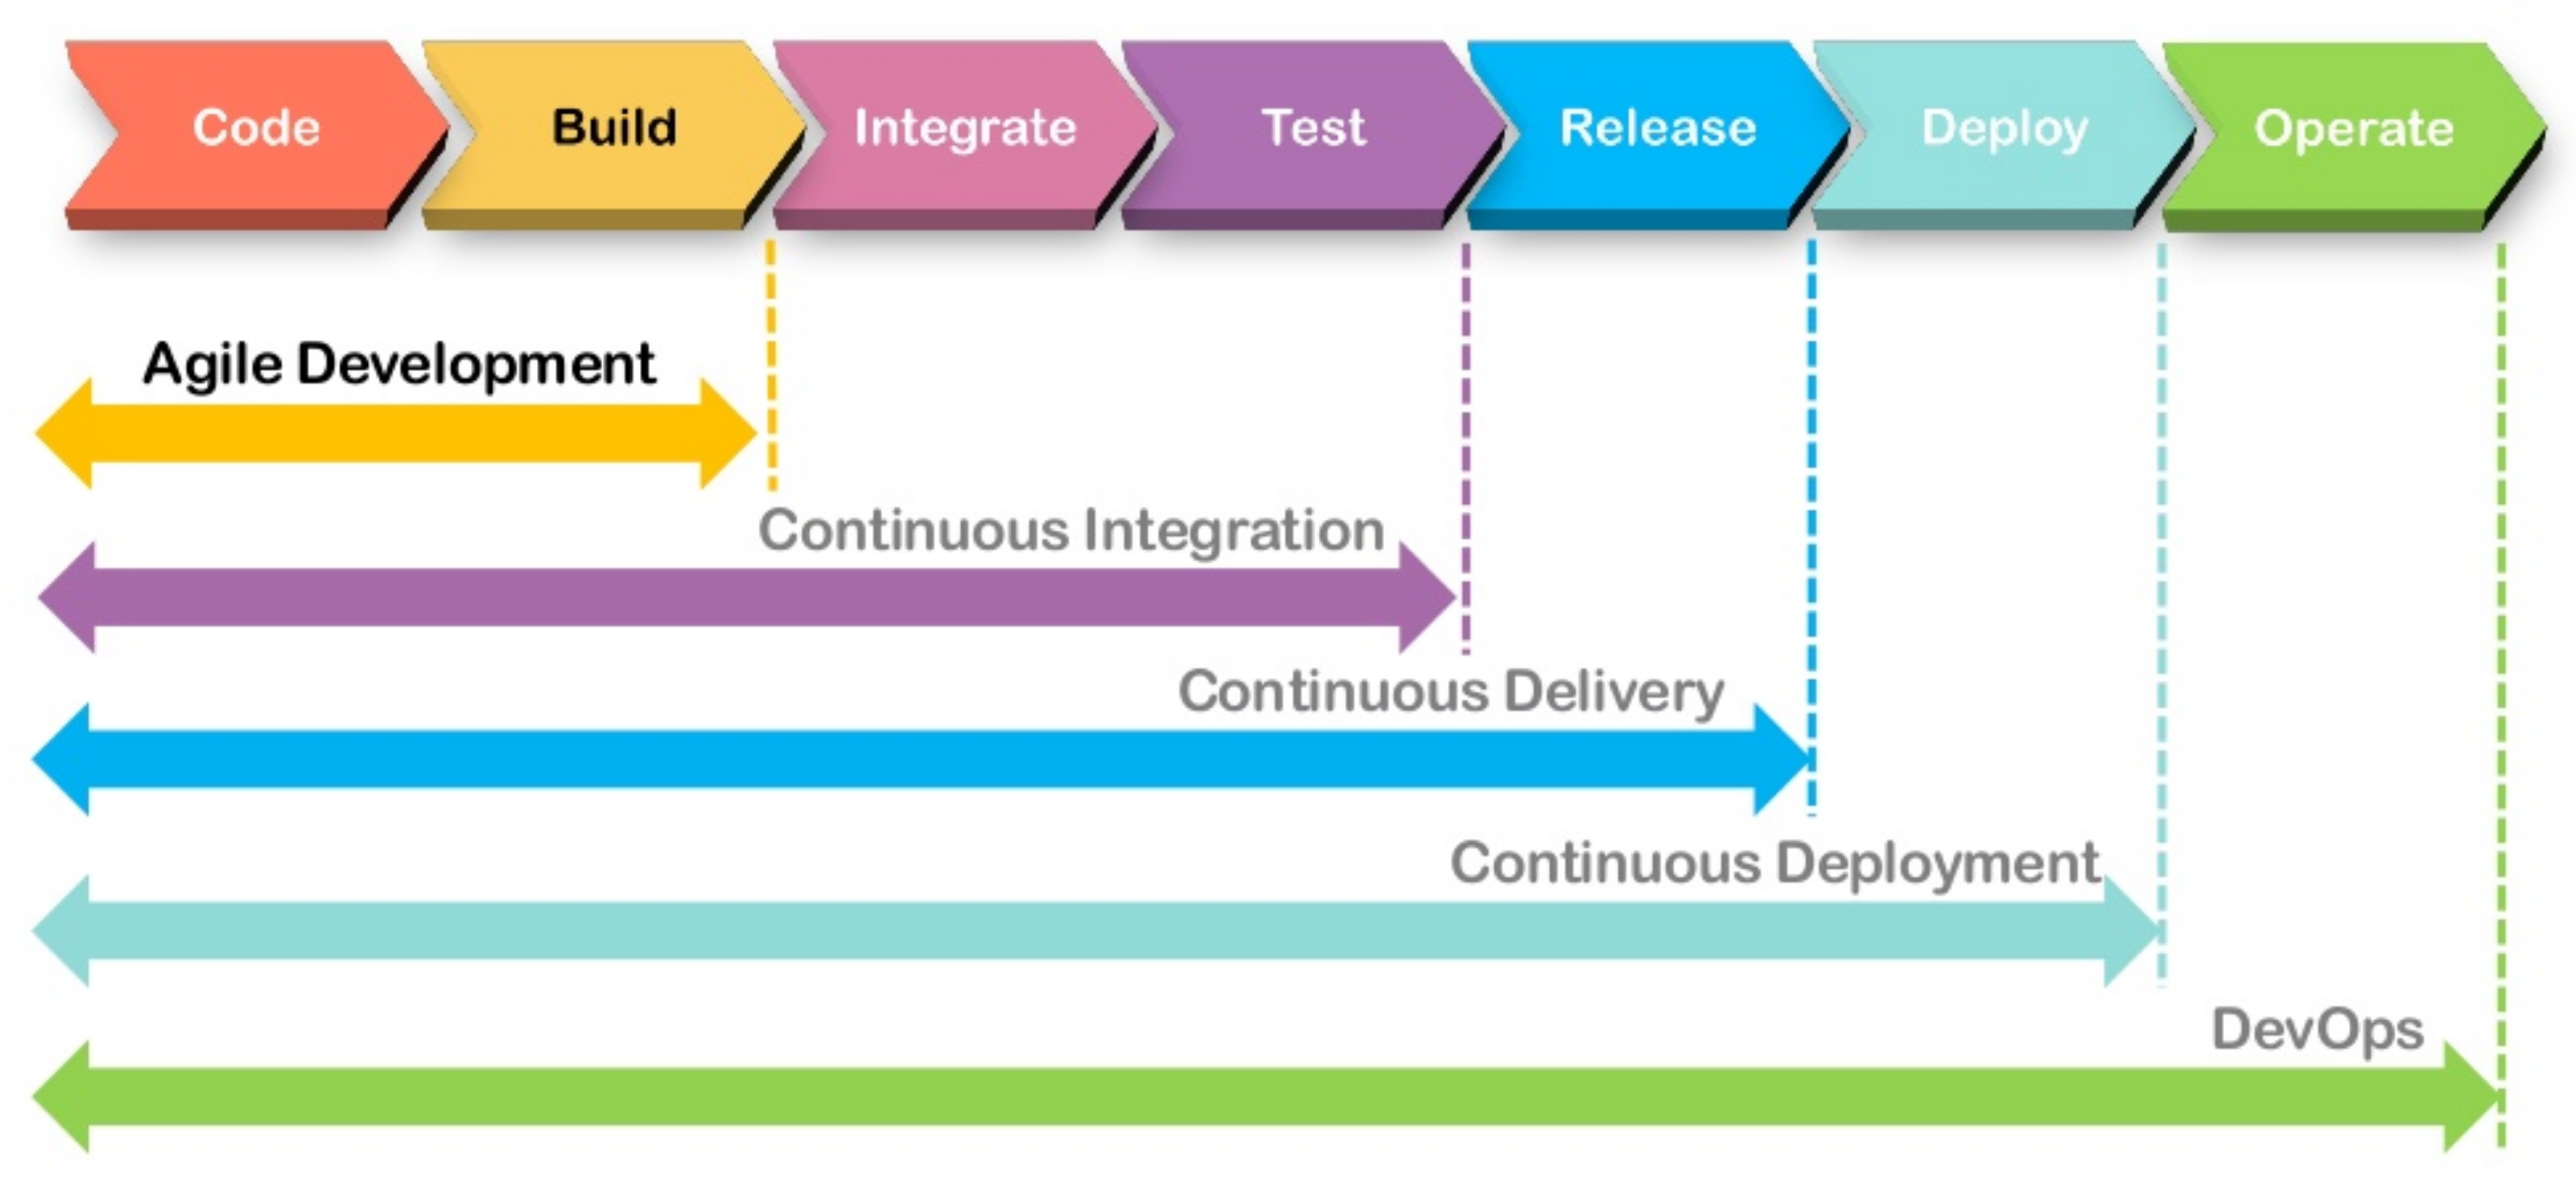
\includegraphics[width=\linewidth]{Images/etapa1}
	\label{fig:etapa1}
\end{figure}
\end{frame}

\begin{frame}{Ejecución - CI/CD}
\begin{figure}
	\centering
	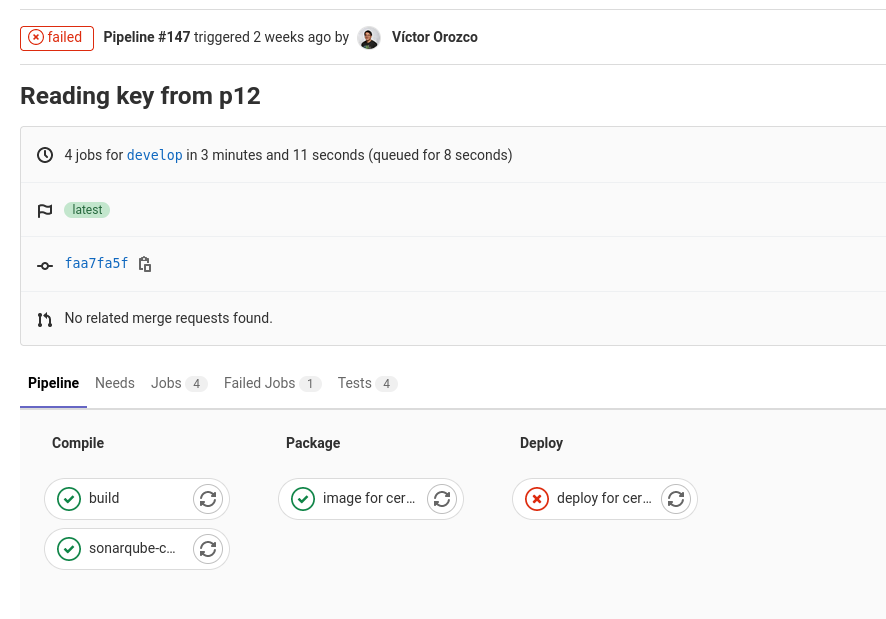
\includegraphics[width=0.8\linewidth]{Images/cicd}
\end{figure}
\end{frame}

\begin{frame}{Control}

\begin{itemize}
\item Tecnológico
    \begin{itemize}
    \item Métricas de calidad del código -e.g. cobertura, code smells, bugs, vulnerabilidades-
    \item Métricas de desempeño -e.g. caídas e intermitencia de red-
    \item Instrumentación de la infraestructura
    \item Monolítos existentes migrados satisfactoriamente
    \end{itemize}
\item  Proyecto
    \begin{itemize}
    \item Presupuesto
    \item Entregables estimados vs plazo
    \item Resultados y percepción de los desarrolladores
    \end{itemize}
\end{itemize}
\end{frame}

\begin{frame}{Control - Calidad}
\begin{figure}
	\centering
	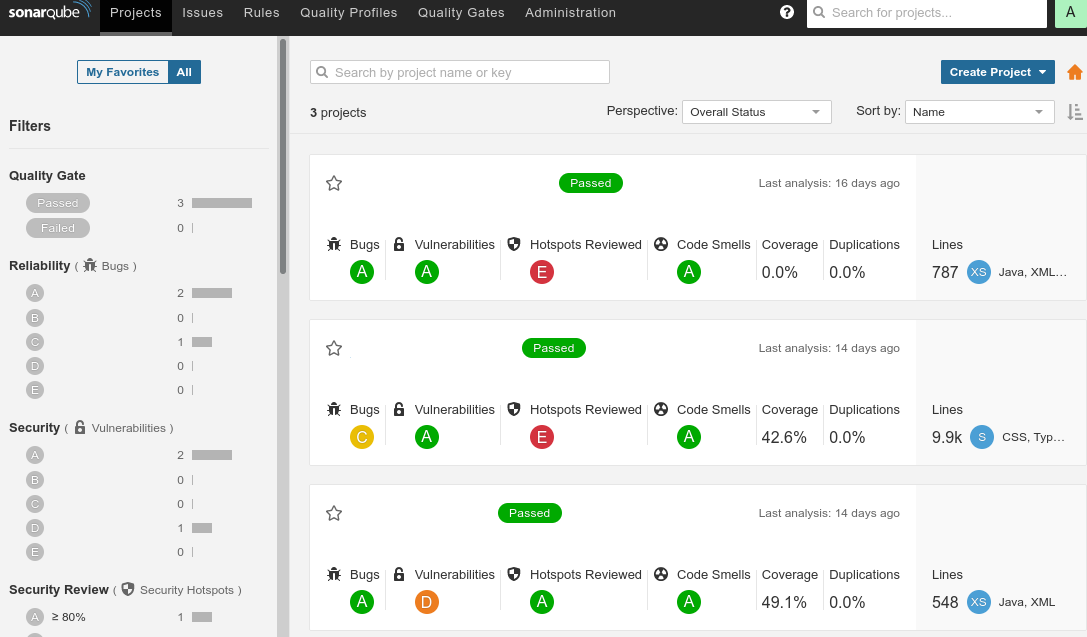
\includegraphics[width=\linewidth]{Images/sonar}
\end{figure}
\end{frame}

\begin{frame}{Control - Instrumentación}
\begin{figure}
	\centering
	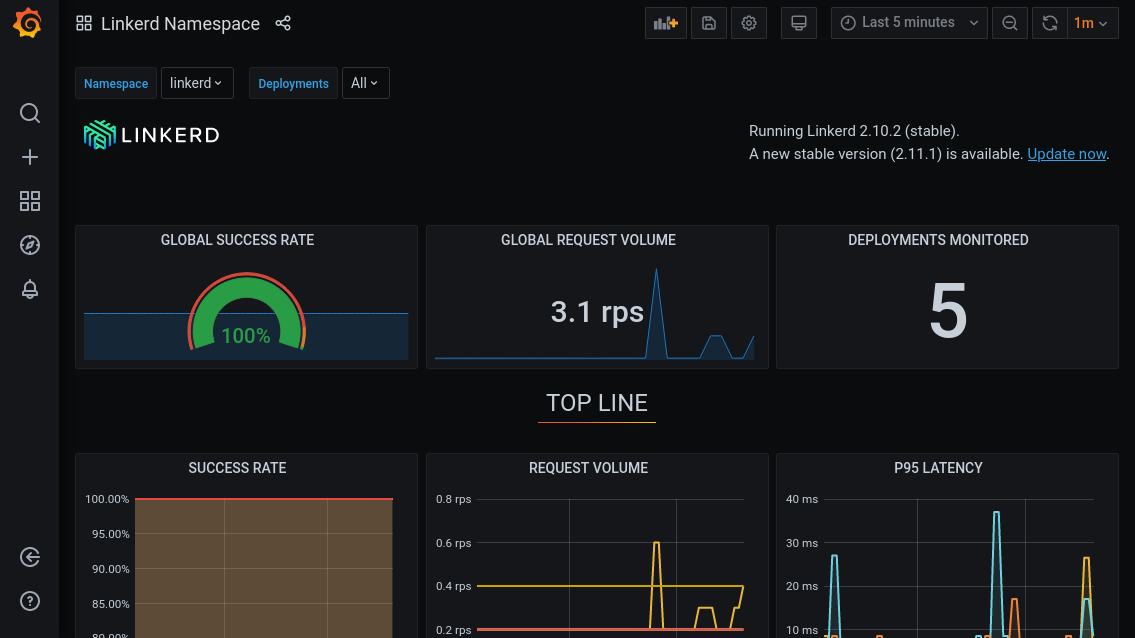
\includegraphics[width=\linewidth]{Images/grafana}
\end{figure}
\end{frame}

\begin{frame}{Cierre}
\begin{itemize}
\item Transición de implementación hacia soporte
\item Documentación viva
\item Propuesta de mejoras
\end{itemize}
\end{frame}

\begin{frame}{Cierre - Documentación viva}
\begin{figure}
	\centering
	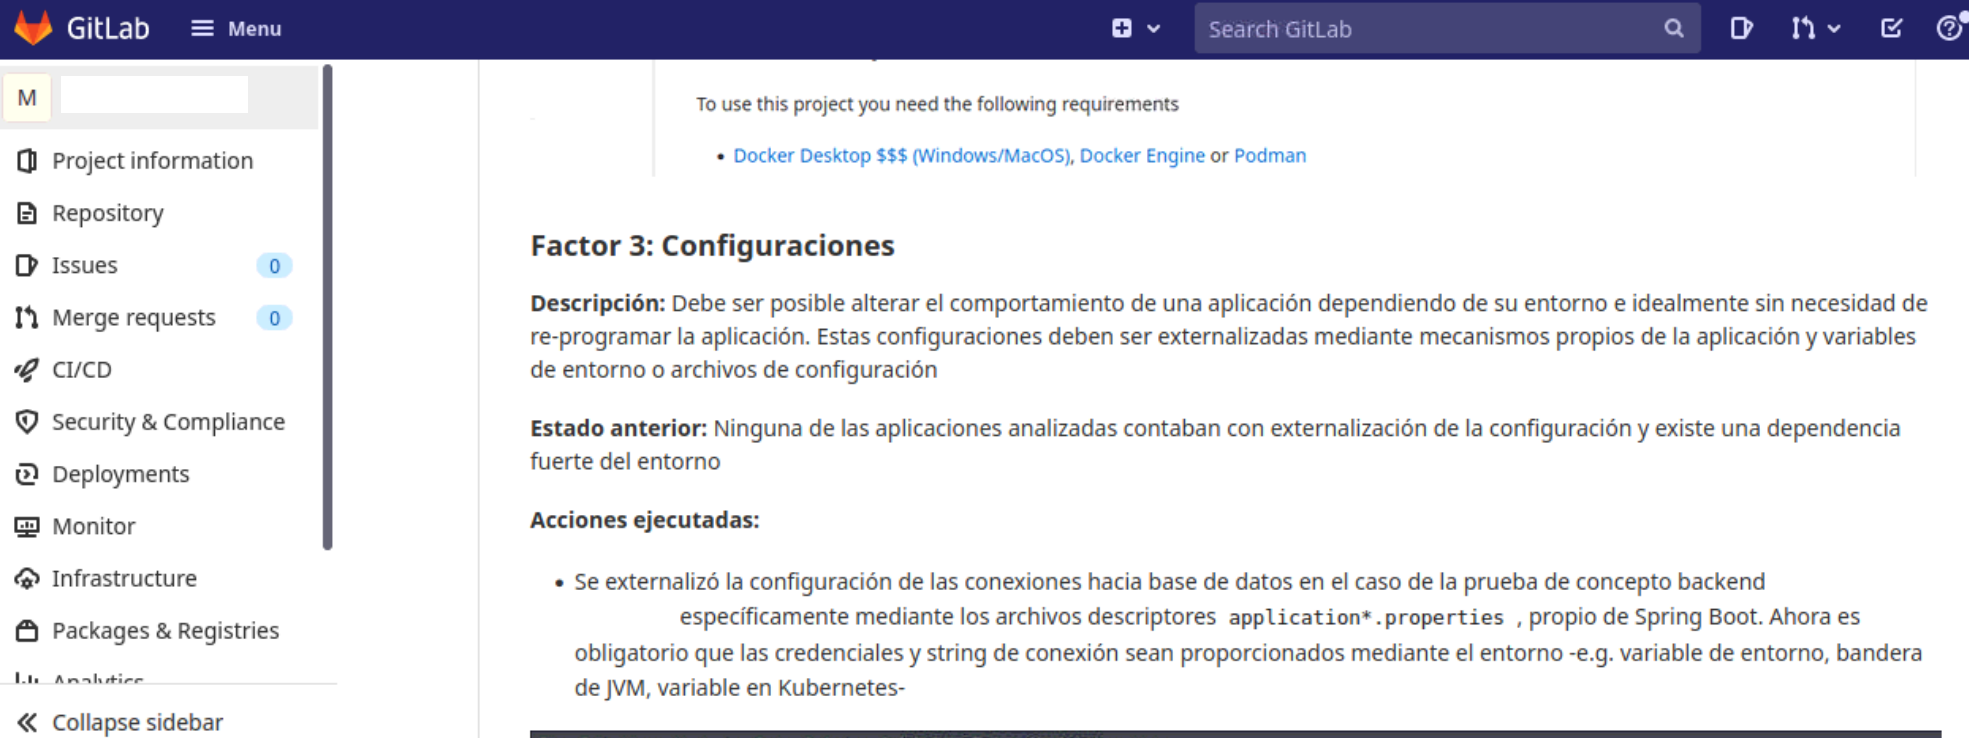
\includegraphics[width=\linewidth]{Images/docviva}
\end{figure}
\end{frame}


\begin{frame}{Víctor Orozco}
    \begin{columns}[T] % contents are top vertically aligned

        \begin{column}[T]{4cm} % alternative top-align that's better for graphics
            \begin{figure}
                \centering
                
\includegraphics[width=\linewidth]{Images/logos}
            \end{figure}
        \end{column}
        \begin{column}[T]{6cm} % each column can also be its own environment
            \begin{itemize}
                \item vorozco@nabenik.com
                \item \href{https://twitter.com/tuxtor}{@tuxtor}
                \item \href{https://vorozco.com}{http://vorozco.com}
                \item \href{https://tuxtor.shekalug.org}{http://tuxtor.shekalug.org}
            \end{itemize}
            \begin{center}
                
\includegraphics[width=0.1\linewidth]{Images/cclogo}
                \\
                This work is licensed under Creative Commons Attribution-NonCommercial-ShareAlike 3.0 Guatemala (CC BY-NC-SA 3.0 GT).
            \end{center}
        \end{column}
    \end{columns}
\end{frame}



\end{document}
